\chapter{About the Authors}\label{chap:About_Authors}
\section*{Alexander Lukens}\label{sec:Alexander_Lukens}
Alexander is an undergraduate engineering student studying towards a Bachelor's Degree in Electrical Engineering at \href{https://www.iit.edu/}{Illinois Institute of Technology}. 
He is entering his final semester of study, with an emphasis on FPGA design and Computer architecture. 
When not pursuing his degree, Alexander works at the \href{https://wiki.ideashop.iit.edu/index.php?title=Main_Page}{Idea Shop Prototyping Lab} where he
helps students from all majors design meaningful models. He is proficient in using electronics prototyping workstations, 3D Printers, Laser Cutters, CNC Mills, and CAD software. My current areas of interest are SoC design and rich web-app development
After graduation, Alexander intends to pursue a graduate degree in Computer Engineering with a focus on integrated circuit design. He is passionate about open source software, and intends to give back to the Computer Engineering community via contributing to open source projects.
\begin{figure}[h!tbp]
  \centering
  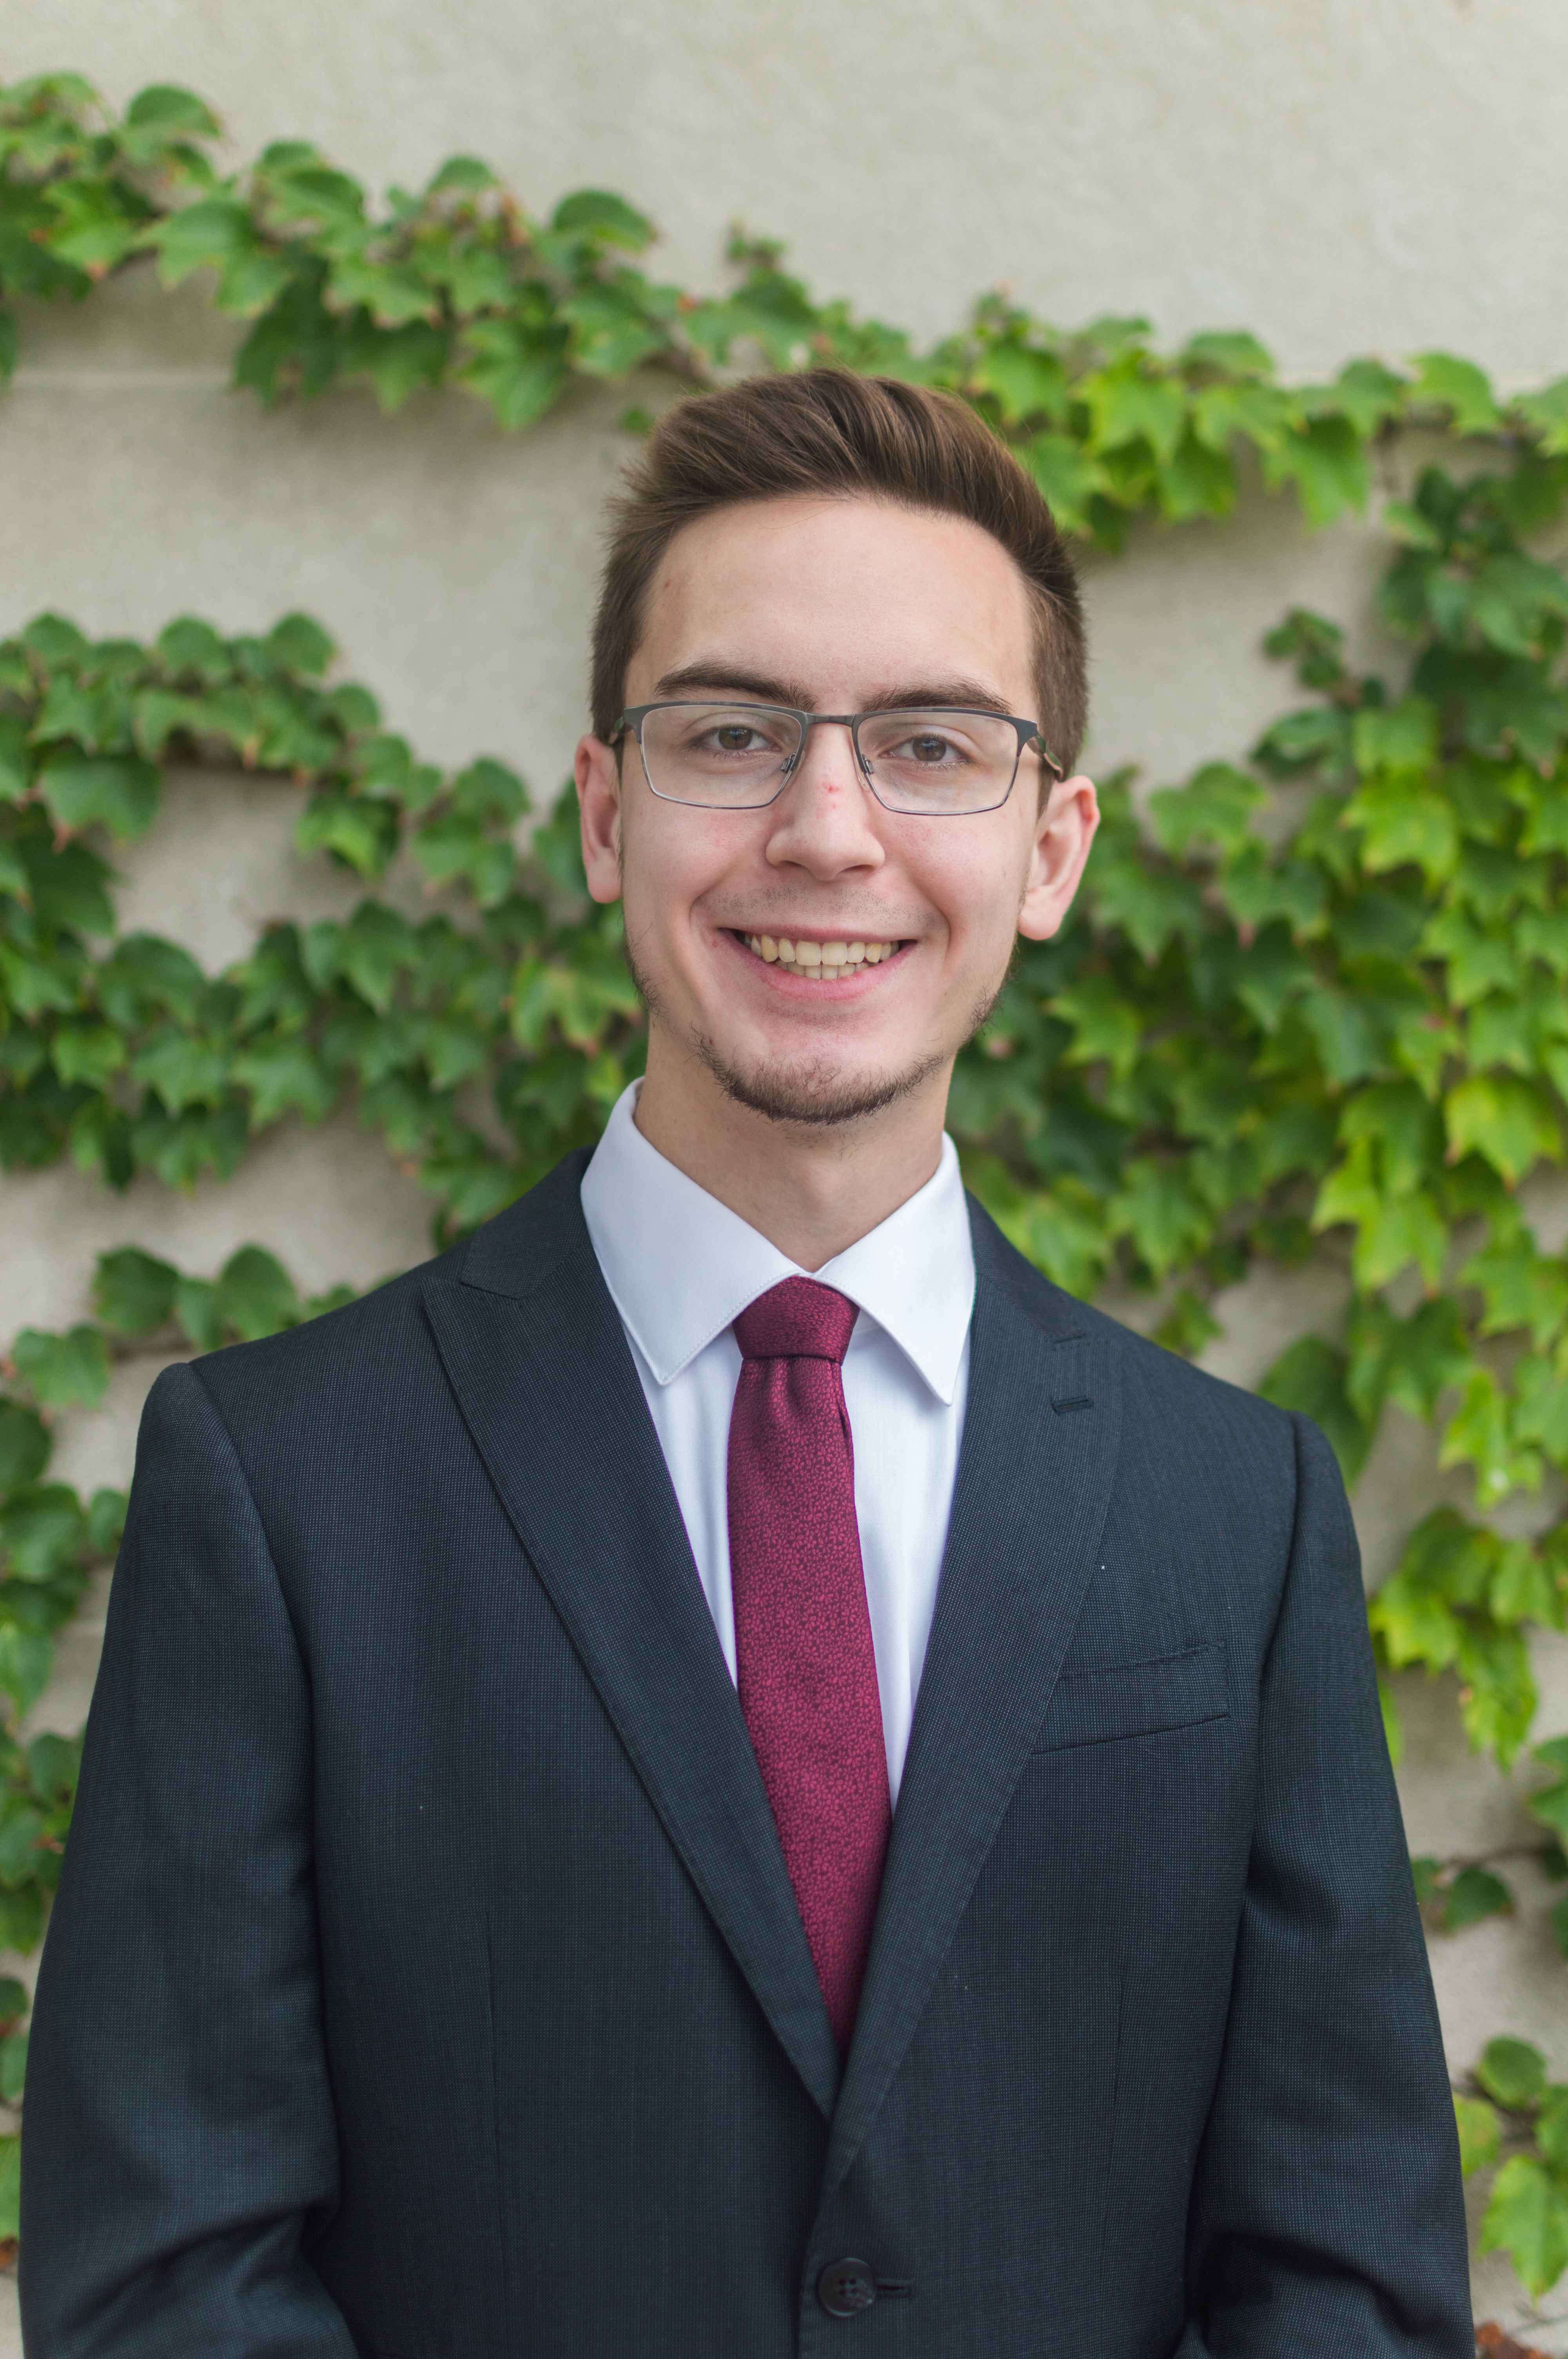
\includegraphics[scale=0.05]{./Lukens_Alex.jpg}
  \caption*{Alexander Lukens}
  \label{fig:Alexander_Lukens}
\end{figure}

\section*{Karl Hallsby}\label{sec:Karl_Hallsby}
Karl is a co-terminal student pursuing his Bachelor's and Master's of Science in Computer Engineering at \href{https://www.iit.edu/}{Illinois Institute of Technology}.
He is currently in his fourth year of undergraduate studies, and is preparing for his graduate work.
He has experience in circuit analysis, hardware design, systems programming, application programming, and programming language theory and design.
Karl is also a member of the CyberHawks cybersecurity student organization, and has been involved in capture-the-flag competitions and protocol analyses.
His professional interests lie in hardware/software co-design, operating systems, and computer cybersecurity, and further extend to programming languages and exotic/novel/esoteric operating systems.

\begin{figure}[h!tbp]
  \centering
  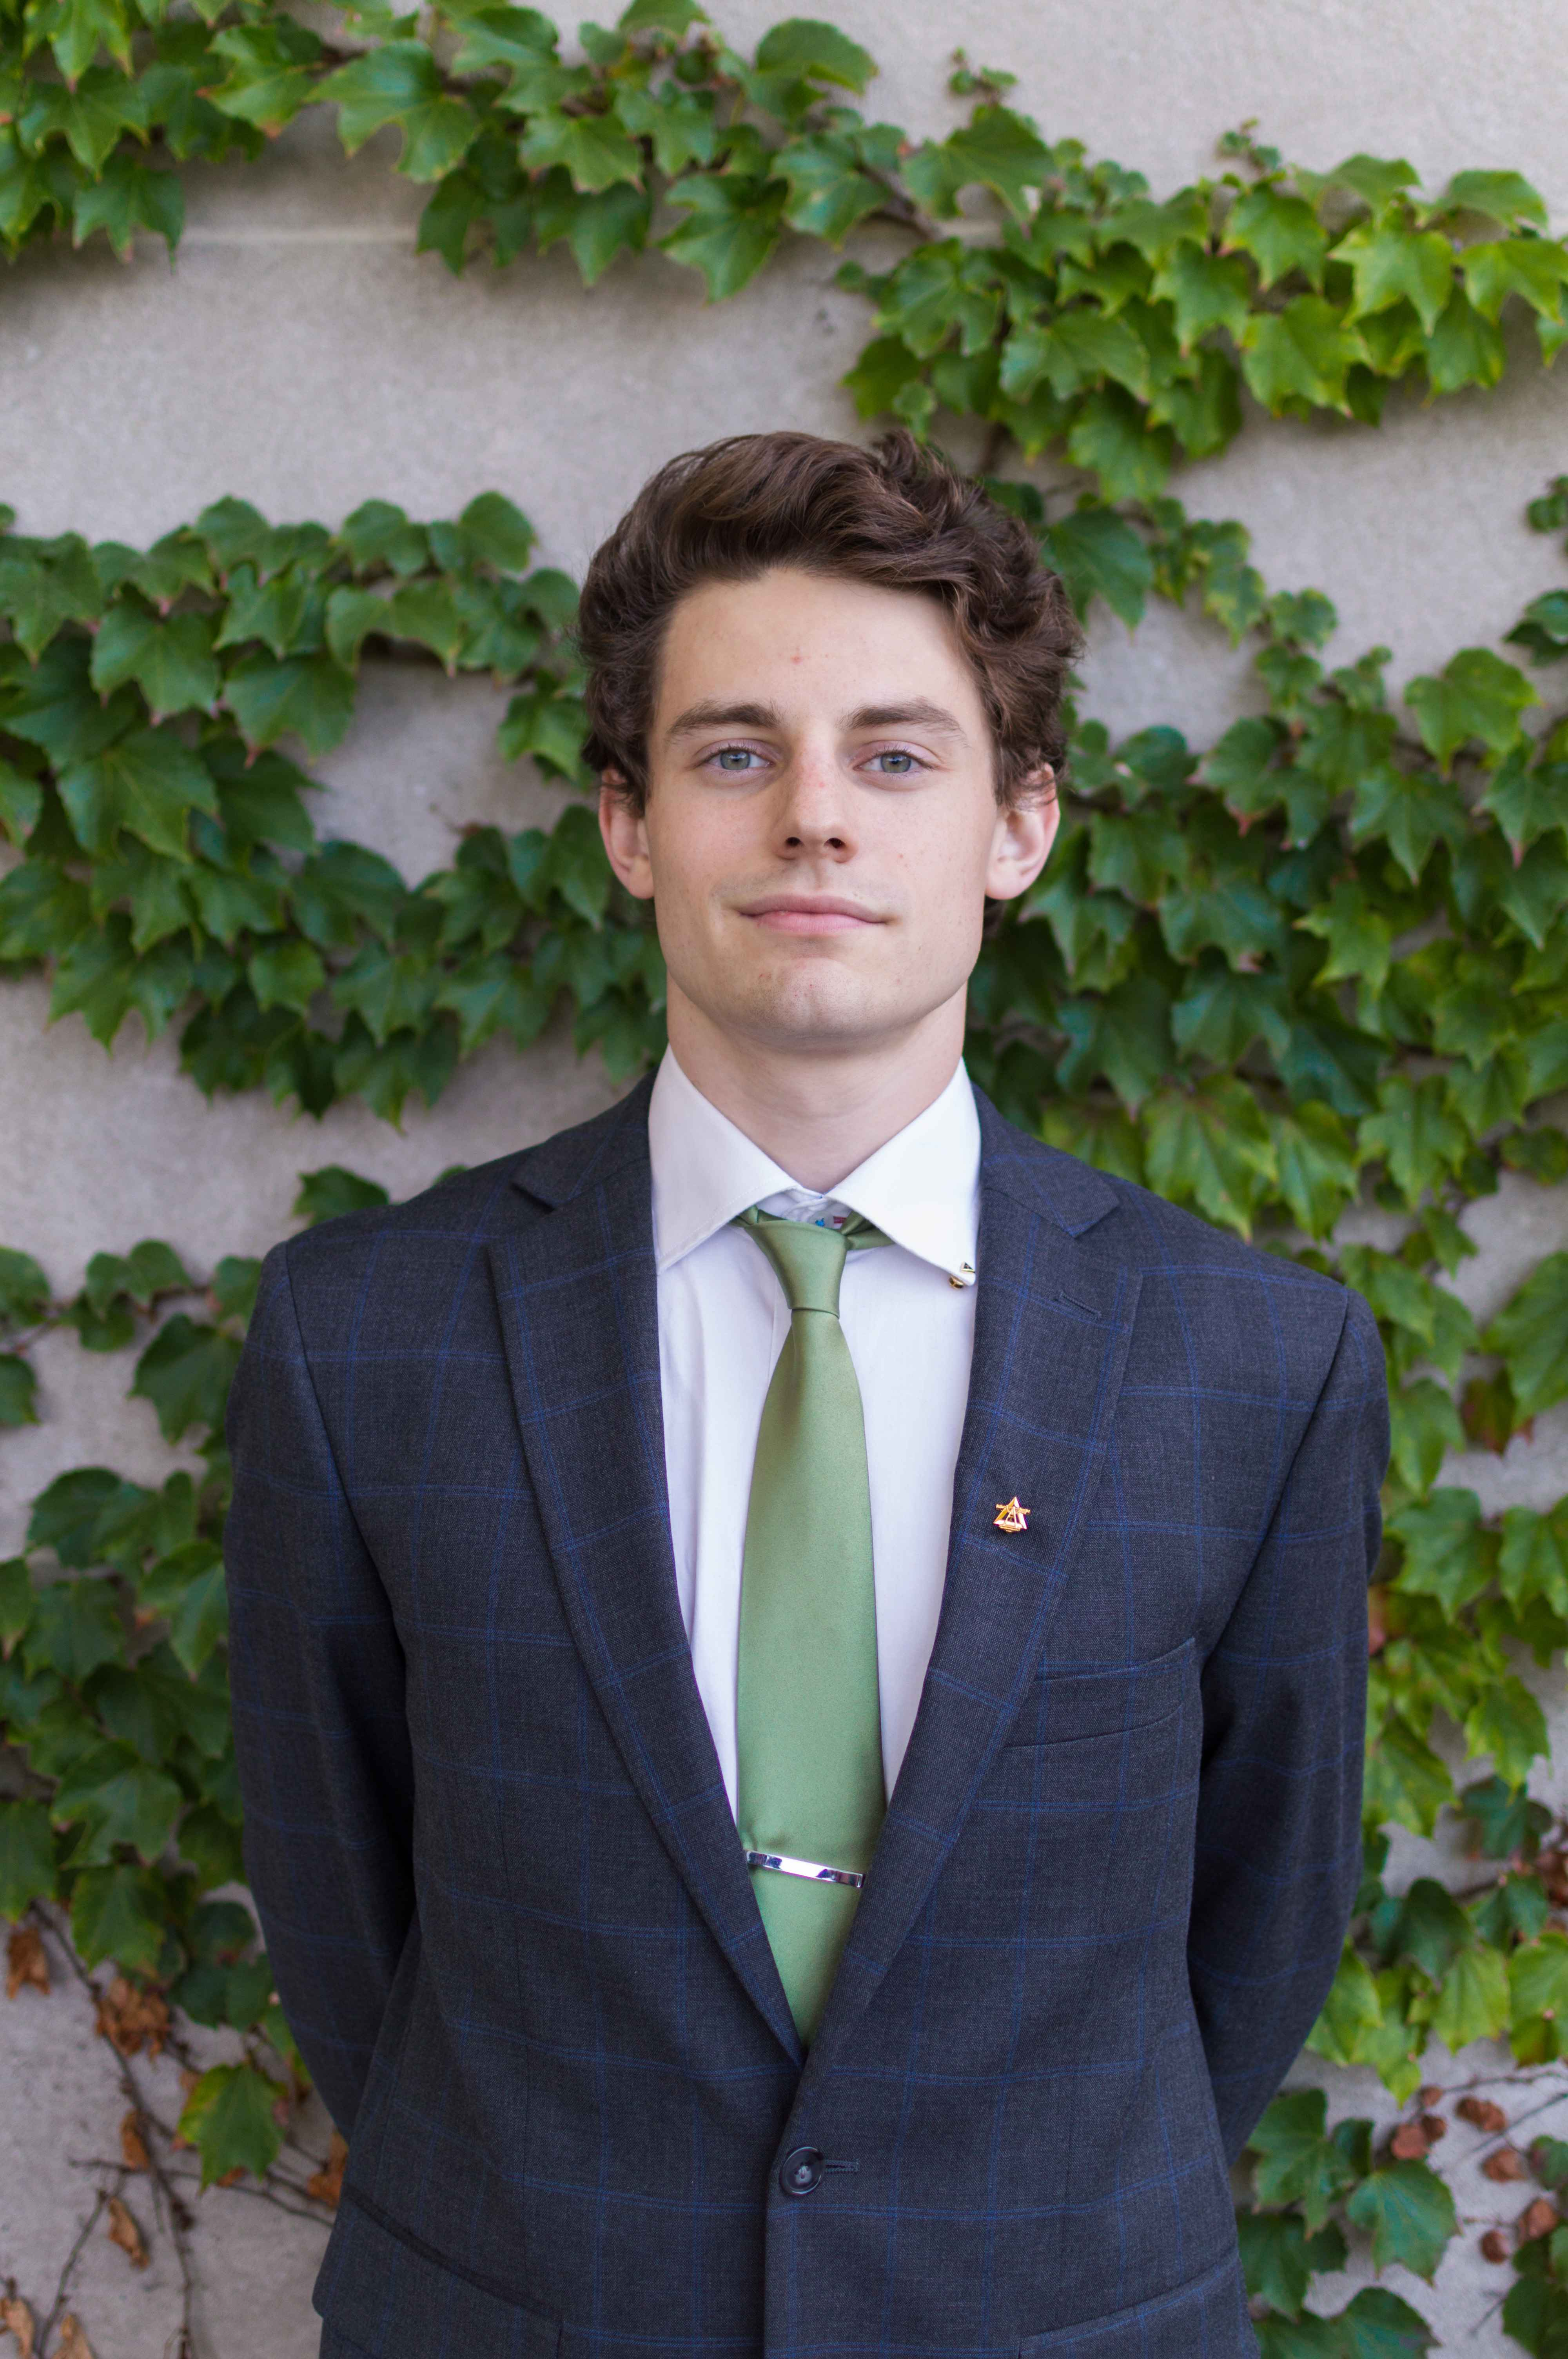
\includegraphics[scale=0.05]{./Hallsby_Karl.jpg}
  \caption*{Karl Hallsby}
  \label{fig:Karl_Hallsby}
\end{figure}

%%% Local Variables:
%%% mode: latex
%%% TeX-master: "../doc"
%%% End:
